\documentclass[10pt]{article}
\usepackage{amsmath,textcomp,amssymb,graphicx,amsthm,enumerate}
\usepackage[top=.75in, bottom=.75in, left=.75in, right=.75in]{geometry}
\newcommand{\argmin}[1]{\underset{#1}{\operatorname{argmin}}\text{ }}
\newtheorem*{theorem}{Theorem}
\newtheorem{lamma}{Lemma}[section]
\theoremstyle{definition}
\newtheorem*{definition}{Definition}
\begin{document}
\title{Fast, Robust Classification with Applications to Periodic Variable Stars}
\author{Siqi Wu, Mark Rogers, and James Long}
\maketitle


\section{Introduction}

\section{The Data}
\subsection{Background on Periodic Variables}
Modern astronomical surveys observe millions of light sources (stars, galaxies, asteroids) over the course of a mission lasting a few years. Periodic variables, sources which vary periodically in brightness over time, are some of the most interesting. In the 1920's, periodic variables were crucial in Edwin Hubble's discovery the existence of galaxies \cite{berendzen1971hubble}. More recently, periodic variables have played an important role in determining expansion of the universe \cite{freedman2010hubble}.

Periodic variables may be divided into a few dozen classes based on physical properties of light sources. Separating the sources into classes is a critical step in turning raw astronomical observations into scientific knowledge. The size of modern data sets requires that much of this work be automated by machine learning and statistical classifiers. 
\begin{figure}[ht]
\begin{minipage}[t]{.45\linewidth}
  \centering
    \begin{includegraphics}[scale=.48]{2000.pdf}
      \caption{Light curve of a Classical Cepheid type variable star. The brightness of the star is on the y-axis. For the top plot the brightness is plotted against time. This time series is periodic. Using fourier methods we can estimate a period of 4.51 days. We can convert the times from the top plot into phase ((time modulo period) / period)). Brightness versus phase is plotted in the bottom plot. Here we can observe the structure in the time series, which is usually similar for stars of the same class but different for stars of different classes.\label{fig:cepheid}}
    \end{includegraphics}
\end{minipage}
\hspace{1cm}
\begin{minipage}[t]{.45\linewidth}
  \centering
    \begin{includegraphics}[scale=.48]{204.pdf}
      \caption{Light curve of a Mira type variable star. Mira variable stars have higher amplitude and longer periods than Cepheid variables. Notice that the period estimate of 322.55 appears to be incorrect. The true period is likely half of this.\label{fig:mira}}
    \end{includegraphics}
\end{minipage}
\end{figure}

Figure \ref{fig:cepheid} displays the light curve (i.e. time series) of a periodic variable belonging to the class Classical Cepheid. The points in the top plot represent flux measurements in magnitudes (i.e. brightness of the source) made by the telescope at particular times. The 0 point on the time axis is arbitrary. Using fourier methods, one can estimate a period using these measurements.  The lower plot of Figure \ref{fig:cepheid} displays the flux measurements of the same object. However here the x-axis is phase of each time measurement, computed using the estimated period of 4.51 days. Here we can observe the structure of the periodic variation. This is known as the \textit{folded light curve}.

Figure \ref{fig:mira} displays an example of a Mira light curve. From the y-axis we can see that this source has higher amplitude than the Classical Cepheid (this is typical of the Mira class) and more sinusoidal variation (also typical). Note that the fourier methods appear to have estimated an incorrect period for this source. The true period appears to be around 161 days, half of the estimate.
\subsection{Classification Methodology}
There has been a lot of recent progress in the astronomy literature towards developing highly accurate classifiers for periodic variables \cite{debosscher2007automated,richards2011machine,dubath2011random}. The standard approach works as follows. A telescope observes a source $j$ at times $t_{1},\ldots,t_{l}$, recording flux measurements of $m_{1},\ldots,m_{l}$. Typically there are measurements of uncertainty on the flux measurements $e_{1},\ldots,e_{l}$. So each source $j$ is initially characterized by an $l \times 3$ matrix $D_j=\{(t_{i},m_{i},e_{i})\}_{i=1}^{l}$. Note that $l$, the number of times the source is observed, is different for each $D_j$. Also the time sampling of the flux measurements is irregular and different for each source. Associated with each source is a classification, such as Mira, Classical Cepheid, RR Lyrae, etc.

In order to construct a classifier, features are \textit{extracted} from $D_j$ (i.e. take functions of $D_j$) that will separate sources into different classes. Features vary from study to study, but typical ones include period (inverse of strongest fourier frequency), amplitude, skew, and estimates of derivatives.

If we compute $p$ features and have a total of $n$ training stars of known class ($D_1, \ldots D_n$), then we can use standard classification techniques on this $n\times p$ data matrix to construct a classifier. Given this classifier, we can then assign a class to a new source by extracting features and running the features through the classifier.


\subsection{Uncertain Features}
\begin{figure}[h]
  \begin{center}
    \begin{includegraphics}[scale=.5]{period_amplitude.pdf}
      \caption{Period-Amplitude relationship for two classes: \textit{Classical Cepheid} stars and \textit{Population II Cepheid} stars. The green box represents (roughly) the physically possible range of periods and amplitudes. Clearly some of these features have been estimated incorrectly.\label{fig:period_amplitude}}
    \end{includegraphics}
  \end{center}
\end{figure}
A major problem with the standard approach is the high levels and heteroskedastic nature of the uncertainty in the features due to having poorly sampled time series ($l$ is small), high error in the flux measurements ($e_{i}$ are systematically large), or irregular nature of sampling ($t_i$'s are highly concentrated, giving a poor representation of variation). This leads to situations where features meant to represent physical quantities of the time series, such as amplitude or period, are incorrect. As an example in Figure \ref{fig:period_amplitude} we plot the period and amplitude features for two classes of stars with a box around known physical limits for these features for these two classes. Some of the observations have values outside these physical limits, clearly indicating that the features are incorrectly estimated. This suggests that classifiers which incorporate feature uncertainty may be able to acheive improved performance.

%% Many of the features used for classification rely on a correct estimate of period for the object. For example, features related to the derivative are often computed based on the folded light curve. If the light curve is folded on the wrong period, then the derivative estimates are likely to be wrong.

\section{SVMs for Interval Data}
Support Vector Machines (SVMs) are a popular method for constructing classifiers. Let $x_i \in \mathbb{R}^p$ be the vector of features for observation $i$ and $y_i$ its class (either $-1$ or $+1$), we can determine the SVM classifier by solving the optimization problem,
\begin{equation}
\label{eq:svm}
\min_{\beta,\beta_0}  \sum_{i=1}^n (1 - y_i(\beta^Tx + \beta_0))_{+} + \frac{\lambda}{2}\beta^T\beta
\end{equation}
The optimal $\beta^*$ and $\beta_0^*$ are used to classify a new observation $x$ using $sign(\beta^* x + \beta_0)$. $\lambda$ is a tuning parameter that balances a tradeoff between maximizing the margin and separating observations in different classes. An optimal $\lambda$ may be chosen using 0-1 loss on a test set or through cross-validation. See \cite{scholkopf2002learning} for an extensive overview of SVMs.

Various extensions to the standard SVM have been proposed that seek to incorporate uncertainty in the features into the optimization problem. These formulations often take (or can be interpreted) as minimizing the objective function for a worst case allocation of features in some fixed set, i.e.
\begin{equation}
\label{eq:svm_minimax}
\min_{\beta,\beta_0}  \max_{z \in \mathcal{X}} \sum_{i=1}^n (1 - y_i(\beta^Tz_i + \beta_0))_{+} + \frac{\lambda}{2}\beta^T\beta
\end{equation}
See \cite{bhattacharyya2004robust,shivaswamy2006second,ben2011chance} for discussions of some of these models.



TO DISCUSS:
\begin{enumerate}
\item similarities to elastic net of LASSO / SVM e.g. Wang \cite{wang2007hybrid}
\item our algorithm is not contained (?) in those considered by Russet \cite{rosset2007piecewise}
\end{enumerate}


\section{Path Algorithm for Interval SVM}


\subsection{Problem formulation}
Suppose $n$ data points are given: $(x_i,y_i)$ for $i=1,...,n$. Let $\mathcal I_+ = \{i: y_i=+1\}$ and $\mathcal I_- = \{i: y_i=-1\}$ be the set of positive class and negative class respectively. Also let $n_+=|\mathcal I_+|$ and $n_-=|\mathcal I_-|$ be the number of data points in these two classes. In this section, we will derive an efficient algorithm to compute the entire regularization path for the following interval SVM problem:
\begin{equation}
\label{eq:svmInit}
\min_{\beta}\sum_{i=1}^n(1-y_i(\beta_0+\beta^Tx_i)+\rho\sigma_i^T|\beta|)_++\frac{\lambda}{2} ||\beta||_2^2.
\end{equation}
%\eqref{eq:q}
%(\ref{eq:q})
Introducing slack variables, the problem becomes:
\begin{align}
\label{eq:primal}
\min & \sum_{i=1}^n\xi_i + \lambda\frac{\beta^T\beta}{2}, \\
\text{subject to } & \xi_i \geq 1 - y_i(\beta_0+\beta^Tx_i)+\rho \sigma_i^Tt,\nonumber \\
                   & \xi_i \geq 0, \text{ for }i=1,2,...,n; \nonumber\\
                   & -t_j\leq \beta_j \leq t_j,\nonumber\\
                   & t_i \geq 0, \text{ for } j=1,2,...,p. \nonumber                      
\end{align}
Let the above problem be the primal problem. The Lagrangian for this problem is
\[
\begin{array}{rl}
L(\xi,\beta_0,\beta,t,\alpha,\gamma,\nu,\mu,c)
%= & \sum_{i=1}^n \xi_i + \lambda \frac{\beta^T\beta}{2} + \sum_{i=1}^n\alpha_i(1 - y_i(\beta_0+\beta^Tx_i)+\rho \sigma_i^Tt-\xi_i) \\
%& - \sum_{j=1}^p\mu_j(t_j-\beta_j) - \sum_{j=1}^p\nu_j(t_j+\beta_j) - \sum_{i=1}^n\gamma_i\xi_i - \sum_{i=1}^nc_jt_j. \\
= & \sum_{i=1}^n(1-\alpha_i-\gamma_i)\xi_i + \lambda\frac{\beta^T\beta}{2} - (\sum_{i=1}^n \alpha_iy_ix_i - (\mu-\nu))^T\beta \\
  & - \sum_{i=1}^n\alpha_iy_i\beta_0 + \sum_{j=1}^p(\rho\alpha_i\sigma_{ji} - \mu_j-\nu_j-c_j)t_j.
\end{array}
\]
Minimizing with respect to the primal variables $(\xi,\beta_0,\beta,t)$, we derive the dual problem as follows:

\begin{align}
\label{eq:dual}
\max_{\alpha,\mu,\nu} & \sum_{i=1}^n \alpha_i - \frac{1}{2\lambda}||\sum_{i=1}^n \alpha_iy_i x_i - (\mu-\nu)||_2^2, \\
\text{subject to } & \sum_{i=1}^n \alpha_i y_i = 0, \ \rho \sum_{i=1}^n \alpha_i \sigma_{i} \geq \mu + \nu, \nonumber \\
& \alpha \in [0,1], \ \mu\geq0, \ \nu\geq0. \nonumber
\end{align}

%Remarks: if the precision matrix $\Sigma$ is zero, the second constraint in the dual problem implies $\mu+\nu\leq0$. In addition, since both $\mu$ and $\nu$ are nonnegative,  we have $\mu=0$ and $\nu=0$. So the dual problem in this case becomes
%\[
%\begin{array}{rl}
%\max_{\alpha} & \sum_{i=1}^n \alpha_i - \frac{1}{2\lambda}||\sum_{i=1}^n \alpha_i y_i x_i||_2^2, \\
%\text{subject to } & \sum_{i=1}^n \alpha_i y_i = 0, \ \alpha \in [0,1],
%\end{array}
%\]
%which is exactly the dual to the standard SVM. See, for example, Equation (12.13) of EML Hastie et al (2009) \cite{hasie2009elements}.\\

One can easily determine the KKT conditions of the interval SVM problem:\\
(1) Primal stationarity:
\begin{align}
\frac{\partial}{\partial \beta}: & \ \beta = \frac{1}{\lambda}(\sum_{i=1}^n \alpha_i y_i x_i + \nu-\mu) \\ 
\frac{\partial}{\partial \beta_0}: & \ \sum_{i=1}^n \alpha_i y_i = 0\\
\frac{\partial}{\partial \xi}: & 1-\alpha - \gamma =0.
\end{align}
(2) Complementary slackness:
\begin{align}
\alpha_i(1 - y_i(\beta_0+\beta^Tx_i)+\rho \sigma_i^Tt-\xi_i) & = 0 \\
\gamma_i\xi_i & = 0 \\
\mu_j(t_j-\beta_j) & = 0 \\
\nu_j(t_j+\beta_j) & = 0 \\
c_jt_j & = 0 \\
\rho \sum_{i=1}^n \alpha_i \sigma_{ji} - (\mu_j +\nu_j+c_j) & =0 
\end{align}
(3) Primal feasibility and; (4) Dual feasibility. Both omitted here due to triviality.\\

From the above optimality conditions, it is easy to observe the following statements hold:\\
(i) If $\xi_i>0$, then $\gamma_i = 0$ and so $\alpha_i =1$. Therefore by (7) we have $y_i(\beta_0+\beta^Tx_i)<1+\rho \sigma_i^Tt$, which indicates that the data point $i$ is on the left of the elbow of the hinge loss. \\
(ii) If $y_i(\beta_0+\beta^Tx_i)> 1+\rho \sigma_i^Tt$, that is, when the $i$-th data point is on the right of the elbow, then $\xi=0$ and by equation (6) and (8) $\alpha_i =0$. \\
(iii) If $y_i(\beta_0+\beta^Tx_i) =  1+\rho \sigma_i^Tt$, that data point is on the elbow. In this case we can only know $\alpha_i\in[0,1]$.\\
%(iv) if $t_j>0$, then $c_j=0$. By equation (XX), $\rho\sum_{i=1}^n \alpha_i \sigma_{ji} = \mu_j+\nu_j$
(iv) It is obvious that at optimal, we have $t = |\beta|$. Hence if $\beta_j>0$ we have $t_j>0$ and so $c_j=0$. On the other hand, since $t_j+\beta_j>0$, $\nu_j=0$. Therefore in this case, $\mu_j = \rho \sum_{i=1}^n \alpha_i \sigma_{ji}$.\\
(v) Similarly, if $\beta_j<0$, $c_j=0$, $\mu_j=0$ and $\nu_j = \rho \sum_{i=1}^n \alpha_i \sigma_{ji}$.\\

Now for convenience let $f(x) = \beta_0+\beta^Tx$ and define the following index sets for the data points:
\[\mathcal E = \{i: y_if(x_i) =  1+\rho \sigma_i^T|\beta|, 0\leq\alpha_i\leq1\}, \ \mathcal E \text{ for Elbow},\]
\[\mathcal L = \{i: y_if(x_i) <  1+\rho \sigma_i^T|\beta|, \alpha_i = 1\}, \ \mathcal L \text{ for Left of the elbow},\]
\[\mathcal R = \{i: y_if(x_i) >  1+\rho \sigma_i^T|\beta|,\alpha_i =0 \}, \ \mathcal R \text{ for Right of the elbow}.\]
Note that the definition of the above sets are similar to those defined in \cite{hastie2004entire} except that we have an extra term $\rho \sigma_i^T|\beta|$ that is related to the uncertainty of the data. In addition, since the absolute value of $\beta$ is involved in our formulation, we also need to keep track of the following index sets for the parameter vector $\beta$:
\[\mathcal V_+ = \{j: \beta_j>0, \nu_j=0\},\]
\[\mathcal V_- = \{j: \beta_j<0,\mu_j=0\},\]
\[\mathcal Z = \{j: \beta_j=0,\sum_{i=1}^n \alpha_i \sigma_{ji} \geq \mu_j + \nu_j\}.\]
\subsection{Initialization}
We will determine the initial state of the parameters and the sets defined above. Without loss of generality, we assume that $n_+\geq n_->0$. We start with $\lambda=+\infty$ or equivalently $C=0$. In this case, it is easy to see that $\beta=0$. 
\begin{lamma}
Given $n_+\geq n_->0$ and $\beta=0$, the optimal value for the initial value of $\beta_0$ is $\beta_0 = 1$ and the loss is $\sum_{i=1}^n \xi_i = 2n_-$. If $n_+>n_-$, then $\beta_0 = 1$.\\
\end{lamma}
\noindent\textbf {Proof.} With $\beta=0$, the primal problem becomes:
\[
\begin{array}{rl}
\min & \sum_{i=1}^n \xi_i, \\
\text{subject to } & \xi_i \geq 0, \ \xi_i \geq 1- y_i \beta_0.
\end{array}
\]
Hence for $i\in \mathcal I_+$, $\xi_i \geq 1-\beta_0$ and for $i\in \mathcal I_-$, $\xi_i \geq 1+\beta_0$. At optimal, the equal sign must hold since we are minimizing the sum $\sum_{i=1}^n \xi_i$. Also, $\xi_i$'s are nonnegative, therefore we have $1-\beta_0\geq0$ and $1+\beta_0\geq0$ and so $\beta_0\in [-1,1]$. Furthermore, the objective function can be written in terms of $n_+$ and $n_-$:
\[
\sum_{i=1}^n \xi_i = n_+(1-\beta_0)+ n_-(1+\beta_0) = (n_--n_+)\beta_0 + (n_++n_-), 
\]
which is a linear function in $\beta_0$. If $n_-=n_+$, then the above function is simply a constant $2n_-$ and so $\beta_0$ can be arbitrary chosen in $[-1,1]$; on the other hand if $n_+>n_-$, the linear function is decreasing in $\beta_0$ and so to minimize the sum, we can pick $\beta_0$ on the right end point of $[-1,1]$. So $\beta_0 = 1$ if $n_+>n_-$. \\

From now on, we can safely assume that $n_+>n_-$, in which case the initial state is $\beta = 0$, $\beta_0=1$, $\xi_i = 0$ for $i\in \mathcal I_+$ and $\xi_i = 2$ for $i\in \mathcal I_-$. Thus by optimality conditions, for any $i\in \mathcal I_-$, $\gamma_i =0$ and so $\alpha_i=1$. In addition, since $0=\sum_{i=1}^n \alpha_i y_i = \sum_{i\in \mathcal I_+} \alpha_i - \sum_{i\in \mathcal I_-} \alpha_i$, we have $\sum_{i\in \mathcal I_+} \alpha_i = \sum_{i\in \mathcal I_-} \alpha_i = n_-$. The following lemma determines the initial value for the dual valuables:
\begin{lamma} Let $\tilde{\beta} = \sum_{i=1}^n \alpha_i y_i x_i + \nu - \mu$, 
\[
\begin{array}{rl}
(\alpha^*,\mu^*,\nu^*) = & \arg\min ||\tilde{\beta}||_2^2, \\
& \text{subject to: } 0\leq \alpha_i\leq 1,  \forall i \in \mathcal I_+; \alpha_i = 1,  \forall i \in \mathcal I_-; \\
& \sum_{i \in \mathcal I_+}\alpha_i = n_-, \rho\Sigma\alpha \geq \mu+\nu, \mu\geq0, \nu\geq0. \\
\end{array}
\]
 and $c^* = \rho\Sigma\alpha^* - \mu^*-\nu^*$. Then for some $\lambda_0$ we have for all $\lambda>\lambda_0$, $(\alpha(\lambda),\mu(\lambda),\nu(\lambda),c(\lambda)) = (\alpha^*, \mu^*,\nu^*,c^*)$.
\end{lamma}  
\noindent\textbf{Proof.} The proof follows directly from Lemma 2 in \cite{hastie2004entire}. The key observasion is that  $\sum_{i=1}^n \alpha_i = 2n_-$ and this sum will remain constant for a while as $\beta$ grows from zero. Then we can plug this sum into the dual problem \eqref{eq:dual} and solve it with additional constraints: $\alpha_i = 1,  \forall i \in \mathcal I_-$ and $\sum_{i \in \mathcal I_+}\alpha_i = n_-$. \\ 

Now let $\beta^* = \sum_{i=1}^n \alpha_i^* y_i x_i + \nu^* - \mu^*$ be the fixed coefficient direction corresponding to the initial $(\alpha^*,\mu^*,\nu^*)$. By the above lemma and the optimality conditions, we have for all $\lambda>\lambda_0$:
\[\beta(\lambda) = \frac{\sum_{i=1}^n \alpha_i^* y_i x_i + \nu^* - \mu^*}{\lambda}.\]
We now need to determine the point $\lambda_0$ that the dual variables $(\alpha,\mu,\nu,c)$ start to change. At the very beginning when $\lambda=+\infty$, there are two possible scenarios:
\begin{itemize}
\item There exist at least two data points in $\mathcal I_+$ with $0<\alpha_i^*<1$. Notice that there cannot be only one such element due to the integer constraint $\sum_{i\in \mathcal I_+} \alpha_i^* = n_-$. 
\item For all $i\in \mathcal I_+$, $\alpha_i^*$ is either 0 or 1.
\end{itemize}
For the first scenario, arbitrary pick an $i_+ \in \mathcal I_+$ such that $0<\alpha_{i_+}^*<1$. Since any of these points will stay in the elbow until a point in $\mathcal I_-$ enters the elbow, we can consider the element in $\mathcal I_-$ that first reaches its margin, i.e. $i_- = \arg \min_{i \in \mathcal I_-} x_i^T\beta^* + \rho \sigma_i^T|\beta^*|$. Therefore at $\lambda=\lambda_0$, as both $i_+$ and $i_-$ are at their respective margin, by the definition of elbow, we have the following system of equations:
\begin{align*}
\begin{cases}
\beta_0+\frac{1}{\lambda}x_{i_+}^T\beta^* =  1+\frac{1}{\lambda}\rho \sigma_{i_+}^T|\beta^*|,\\
\beta_0+\frac{1}{\lambda}x_{i_-}^T\beta^* =  -1-\frac{1}{\lambda}\rho \sigma_{i_-}^T|\beta^*|.
\end{cases}
\end{align*}
Solving for $\lambda$ and $\beta_0$ yields:
\begin{align}
\begin{cases}
\lambda_0 = \frac{1}{2}(\beta^{*T}(x_{i_+}-x_{i_-})-\rho|\beta^*|^T(\sigma_{i_+}+\sigma_{i_-})),\\
\beta_0 = \frac{-\beta^{*T}(x_{i_+}+x_{i_-})+\rho|\beta^*|^T(\sigma_{i_+}-\sigma_{i_-})}{\beta^{*T}(x_{i_+}-x_{i_-})-\rho|\beta^*|^T(\sigma_{i_+}+\sigma_{i_-})}.
\end{cases}
\end{align}
For the second scenario, for the initial parameter to change, a point in $\mathcal I_-$ and a point in $\mathcal I_+$ with $\alpha_i^* = 1$ must reach the margin simultaneously. Therefore we can let $i_+ = \arg \max_{i\in \mathcal I_+, \alpha_i=1} x_i^T\beta^* - \rho \sigma_i^T|\beta^*|$ and obtain $\lambda_0$ and $\beta_0$ by solving the above equations.\\

%Remarks: in \cite{hastie2004entire}, Hastie et.al. split the initialization step into two cases depending on whether $n_+=n_-$ or $n_+>n_-$. In their case $n_+=n_-$, the initial state can be obtained efficiently without solving the quadratic programming problem. This does not seem to be the case in our problem, as it also involves finding the initial values of the extra dual variables $\mu$ and $\nu$. Therefore solving a quardratic problem for starting up the path algorithm cannot be avoided in our case.\\

\subsection{The Path}
As in \cite{hastie2004entire}, our algorithm keeps track of the following events:
\begin{enumerate}
\item[1.] One or more points from $\mathcal L$ have just entered $\mathcal E$;
\item[2.] One or more points from $\mathcal R$ have just reentered $\mathcal E$;
\item[3.] One or more points in $\mathcal E$ have just left the set, to join either $\mathcal R$ or $\mathcal L$.
\end{enumerate}
\noindent In addition, we also need to keep track of the following events involving the sign of the components of $\beta$:
\begin{enumerate}
\item[4.] One or more indices of the parameter $\beta$ enter $\mathcal Z$, that is,  $\beta_j$ becomes zero, initially being either positive or negative;
\item[5.] One or more indices of the parameter $\beta$ enter $\mathcal V_+$ from $\mathcal Z$;
\item[6.]  One or more indices of the parameter $\beta$ enter $\mathcal V_-$ from $\mathcal Z$.
\end{enumerate}
\subsection{Piecewise Linearity between Events}
By continuity, all of the index sets defined will stay the same until the next event occurs. Index by the superscript $l$ the sets immediately after the $l$-th event occurs. Likewise, index all the parameters in the same manner, and let $f^l$ be the classify function at this point. Also, for notation consistency define $\alpha_0 = \lambda \beta_0$ and so $\alpha_0^l = \lambda^l \beta_0^l$. Consider for $\lambda^l > \lambda > \lambda^{l+1}$, we have:
\begin{align}
\label{eq:classifier}
f(x) & = [f(x) - \frac{\lambda^l}{\lambda}f^l(x)] + \frac{\lambda^l}{\lambda}f^l(x) \nonumber \\
%& = \frac{1}{\lambda}[x^T(\sum_{i=1}^n\alpha_iy_ix_i+\nu-\mu)+\alpha_0 - x^T(\sum_{i=1}^n\alpha_i^ly_ix_i+\nu^l-\mu^l)-\alpha_0^l+\lambda^l f^l(x)] \nonumber \\
& = \frac{1}{\lambda}[x^T\sum_{i\in\mathcal E^l}(\alpha_i-\alpha_i^l)y_ix_i+x^T(\nu-\nu^l)-x^T(\mu-\mu^l)+(\alpha_0-\alpha_0^l) +\lambda^l f^l(x)],
\end{align}
where the last equality follows from the fact that $\{1,...,n\}=\mathcal L\cup\mathcal E\cup \mathcal R$, $\alpha_i = 1$ on $\mathcal L$ and $\alpha_i=0$ on $\mathcal R$. The value of $\alpha_i$ for $i$ not in the elbow remains unchanged between events. Since each data point in $\mathcal E^l$ is to stay in $\mathcal E$ for $\lambda\in (\lambda^{l+1},\lambda^{l})$, we have:
\[y_jf(x_j) = 1+ \rho\sigma_j^T|\beta|, \forall j\in\mathcal E.\]
Plug in \eqref{eq:classifier} for $f(x_j)$, the above equation becomes:
\begin{align}
\label{eq:elbow}
\frac{1}{\lambda}[\sum_{i\in\mathcal E^l}(\alpha_i-\alpha_i^l)y_jy_ix_j^Tx_i+y_jx_j^T(\nu-\mu-(\nu^l-\mu^l))+y_j(\alpha_0-\alpha_0^l) +\lambda^l (1+\rho \sigma_j^T|\beta^l|)] = 1+\rho\sigma_j^T|\beta|.
\end{align}
We can expression the parameter $\beta_i$ in terms of $\alpha$. For any $i\in\mathcal V_+^l$, since $\nu_i=0$, $\mu_i = \rho\sum_{k=1}^n \alpha_k\sigma_{ik}$. Plug all these parameters into the formula for $\beta_i$, we have
\[
\beta_i = \frac{1}{\lambda}\sum_{k=1}^n(\alpha_iy_kx_{ik}-\mu_i) =\frac{1}{\lambda}\sum_{k=1}^n\alpha_k(y_kx_{ik}-\rho\sigma_{ik}) = \frac{1}{\lambda}\sum_{k=1}^n\alpha_kw_{ik},\]
where $w_{ik} =y_kx_{ik}-\rho\sigma_{ik}$. Similarly, for $i\in\mathcal V_-$, since $\mu_i=0$, $\nu_i = \rho\sum_{k=1}^n \alpha_k\sigma_{ik}$ and so
\[
\beta_i = \frac{1}{\lambda}\sum_{k=1}^n(\alpha_iy_kx_{ik}+\nu_i) =\frac{1}{\lambda}\sum_{k=1}^n\alpha_k(y_kx_{ik}+\rho\sigma_{ik})=\frac{1}{\lambda}\sum_{k=1}^n\alpha_kz_{ik}.\]
Let $h_{jk} = \sum_{i\in\mathcal V_+^l}\sigma_{ij}w_{ik} - \sum_{i\in\mathcal V_-^l}\sigma_{ij}z_{ik}$. By splitting $\beta$ into positive and negative parts, we have:
\[
\begin{array}{rl}
\sigma_j^T|\beta| &= \sum_{i\in\mathcal V_+^l}\sigma_{ij}\beta_{i} - \sum_{i\in\mathcal V_-^l}\sigma_{ij}\beta_{i} \\
&=\frac{1}{\lambda}\sum_{k=1}^n\alpha_k(\sum_{i\in\mathcal V_+^l}\sigma_{ij}w_{ik} - \sum_{i\in\mathcal V_-^l}\sigma_{ij}z_{ik})\\
&=\frac{1}{\lambda}\sum_{k=1}^n\alpha_kh_{jk}.
\end{array}
\] 
Next, look at the term $x_j^T(\nu-\mu)$. Notice that:
\[
\begin{array}{rl}
x_j^T(\nu-\mu) %& = \sum_{i\in\mathcal V_-^l}x_{ij}\nu_i - \sum_{i\in\mathcal V_+^l}x_{ij}\mu_i + \sum_{i\in Z^l}x_{ij}(\nu_i-\mu_i)\\
& = \sum_{i\in\mathcal V_-^l}x_{ij}(\rho\sum_{k=1}^n\alpha_k\sigma_{ik}) - \sum_{i\in\mathcal V_+^l}x_{ij}(\rho\sum_{k=1}^n\alpha_k\sigma_{ik}) + \sum_{i\in Z^l}x_{ij}(\nu_i-\mu_i)
\end{array}
\]
Observe that for $i\in Z^l$, $\beta_i=0$ and so $\sum_{k=1}^n\alpha_ky_kx_{ik}+\nu_i-\mu_i=0$. Therefore $\nu_i-\mu_i = -\sum_{k=1}^n\alpha_ky_kx_{ik}$. Hence we have:
\[
x_j^T(\nu-\mu) = \sum_{k=1}^n\alpha_k(\rho\sum_{i\in\mathcal V_-}x_{ij}\sigma_{ik}-\rho\sum_{i\in\mathcal V_+}x_{ij}\sigma_{ik}+\sum_{i\in Z}y_kx_{ik}) = \sum_{k=1}^n\alpha_k g_{jk},
\]
where $g_{jk}=\rho\sum_{i\in\mathcal V_-^l}x_{ij}\sigma_{ik}-\rho\sum_{i\in\mathcal V_+^l}x_{ij}\sigma_{ik}+\sum_{i\in Z^l}y_kx_{ik}$. Now, let $\delta_k = \alpha_k^l-\alpha_k$. After some rearrangements, Equation \eqref{eq:elbow} becomes:
\[
\sum_{k\in\mathcal E}\delta_k(y_jy_kx_j^Tx_k + y_j g_{jk} - \rho h_{jk}) + y_j\delta_0 = \lambda^l-\lambda,
\]
for all $j\in\mathcal E$. Thus following \cite{hastie2004entire}, by constructing a matrix $\mathbf{K}$ with entry $K_{jk} = y_jy_kx_j^Tx_k + y_j g_{jk} - \rho h_{jk}$, the above system of equations can be written:
\[
\mathbf{K}\boldsymbol{\delta} + \delta_0 \mathbf{y}_l = (\lambda^l-\lambda)\textbf{1},
\]
where $\mathbf{y}_l$ is a vector of length $m$ whose entries are $y_i$'s for $i\in \mathcal E^l$. In addition, since $\sum_{i=1}^n \alpha_iy_i = 0$, we have $\sum_{k\in\mathcal E}y_k\delta_k=0$ and so
\[\mathbf{y}_l^T\boldsymbol{\delta}=0.\]
So all together we have $m+1$ unknown variables and $m+1$ linear equations. Now let:
\[
\mathbf{A}_l = 
\left( \begin{array}{cc}
0 & \mathbf{y}_l^T \\
\mathbf{y}_l & \mathbf{K}_l 
\end{array}\right), \
\boldsymbol{\delta}^a = 
\left( \begin{array}{c}
\delta_0 \\
\boldsymbol{\delta}
\end{array}
\right), \ 
\textbf{1}^a = 
\left( \begin{array}{c}
0 \\
\textbf{1}
\end{array}
\right). 
\]
So the linear system can be written as
\[
\mathbf{A}_l\boldsymbol{\delta}^a = (\lambda_l-\lambda)\textbf{1}^a.
\]
Let $\textbf{b}^a = \mathbf{A}_l^{-1}\textbf{1}^a$, then for $k=0$ or $k \in \mathcal E^l$, we have
\begin{align}
\label{eq:alpha}
\alpha_k = \alpha_k^l - (\lambda^l-\lambda)b_k,
\end{align}
which shows linearity of $\alpha$ between two events, i.e. $\lambda^{l+1}<\lambda<\lambda^{l}$. To evaluate the function value of $f$ at the data point $x_j$, we have
\begin{align}
\label{eq:fxj}
f(x_j) = \frac{\lambda^l}{\lambda}(f^l(x_j)-h^l(x_j))+h^l(x_j),
\end{align}
where $h^l(x) = \sum_{k\in\mathcal E_l}b_j(y_kx_j^Tx_k+g_{jk})+b_0$.

\subsection{Finding the Next Event}
The linear path established above continues until one of the following events occur:
\begin{enumerate}
\item One of the points (if any) on the elbow $\mathcal E^l$ is about to enter either $\mathcal R$ ($\alpha_i=0$) or $\mathcal L$ ($\alpha_i=1$). By solving equation \eqref{eq:alpha} we can obtain a candidate breakpoint $\lambda$ for the $j$-th data point to enter the respectively $\mathcal R$ and $\mathcal L$:
\[
\lambda = \frac{\lambda^lb_j-\alpha_j^l}{b_j} \text{ and } \lambda = \frac{\lambda^lb_j-\alpha_j^l+1}{b_j}.
\]
%Compute the above candidate break points for all data points that are currently on the elbow (so that we have $2m$ such candidates). Take the greatest such $\lambda$ that is smaller than $\lambda^l$, denote that quantity by $\lambda_a$.
\item One of the points $j$ in either $\mathcal L^l$ or $\mathcal R^l$ enters the elbow, that is $y_jf(x_j) = 1+\rho\sigma_j^T|\beta|$. By Equation \eqref{eq:fxj}, we have
\[
\frac{\lambda^l}{\lambda}(f^l(x_j)-h^l(x_j))y_j + h^l(x_j)y_j = 1 + \frac{1}{\lambda}\sum_{i=1}^n\alpha_kh_k.
\]   
%The right-hand-side of the above equation can be rewritten as
%\[
%1+\frac{1}{\lambda}\sum_{k\in\mathcal L^l}h_k + \frac{1}{\lambda}\sum_{k\in\mathcal E^l}(\alpha_k^l + (\lambda-\lambda^l)b_k)h_k.
%\]
Solving the above equation for $\lambda$, we have:
\[
\lambda = \frac{\lambda^l(f^l(x_j)-h^l(x_{jk}))-y_j\sum_{k\in\mathcal L^l}h_{jk} - y_j\sum_{k\in\mathcal E^l}\alpha_k^lh_{jk} + \lambda^l\sum_{k\in\mathcal E^l}b_k h_{jk}}{y_j-h^l(x_j)+y_j\sum_{k\in\mathcal E^l}b_kh_{jk}}.
\]
\item A nonzero component of $\beta$ becomes zero. This means for each $i\in\mathcal V_+^l$, by equation  we solve $\sum_{k=1}^n\alpha_kw_{ik}=0$ and obtain a break point candidate
\[
\lambda = \frac{\lambda^l\sum_{k\in\mathcal E^l} b_kw_{ik}-\sum_{k\in\mathcal E^l}\alpha_k^l w_{ik}-\sum_{k\in\mathcal L^l} w_{ik}}{\sum_{k\in\mathcal E^l} b_kw_{ik}}.
\]
For $i\in\mathcal V_-^l$, simply replace $w_{ik}$ by $z_{ik}$.

\item A zero component of $\beta$ becomes nonzero. For a component $i\in Z^l$ to become positive, we require $c_i = 0$ and $\nu_i =0$, therefore $\mu_i = \sum_{k=1}^n\alpha_ky_kx_{ik}$. Together with the optimality conditions, we need to solve $\rho\sum_{k=1}^n\alpha_k\sigma_{ik}=\sum_{k=1}^n\alpha_ky_kx_{ik}$. Same analysis for $i\in Z^l$ to become negative. The formula for $\lambda$ turns out to have the same form as that in 3.



\end{enumerate}
  
Compute the all of the above $\lambda$'s and take the greatest such $\lambda$ that is smaller than $\lambda^l$. That $\lambda$ will be the break point for the next event. 

\subsection{Continuation and termination}
After finding the $\lambda$ at which the next event occurs, we can update all the index sets accordingly and continue to find the next event. If the data points are separable in the sense of interval data (that is, there is a hyperplane that separates all the rectangles formed by the data points in the two classes), the algorithm can terminate once $\mathcal L^l$ becomes empty. If the points are not separable, then we rely on the user to provide an upper bound or $\lambda$ or a maximum number of break points.

\subsection{A simple simulated example}
To test the correctness and efficiency of our proposed algorithm, we construct a test data set as follows: let $n_+=10$ and $n_-=8$, and to keep the example simple let us consider having only $p=5$ features. For each $i\in\mathcal V_+$ and $j=1,...,5$, generate $x_{ij}$ from a standard normal distribution $N(0,1)$, independently of each other. Similarly, generate each $x_{ij}$ in the negative class from the normal distribution $N(-0.5,1)$. To construct the precision matrix, for each entry in that matrix, simulate a number from $N(0.1,0.1)$ and then take the absolute value of it. Also, we set $\rho = 1.0$ and target the range of $C$ to be $[0,3]$. First, we use a brute-force algorithm to compute the regularization paths for the parameters, making a call to the function that solves one interval SVM problem ({\tt svmInterval}) at a finite break points of along the interval $[0,3]$. We then run our interval SVM path algorithm on this data set and compare the results of the two approaches. The paths for $\beta$ are shown in Figure~\ref{fig:betaPath} and the plots for $\beta_0$ and $\alpha$ can be found in the Appendix. In each of the plot, the paths are computed via the brute-force algorithm and the break points (indicated by the dash lines) are predicted by the path algorithm. It can be seen that our path algorithm correctly identifies all the changing points in this example.


\begin{center}
\begin{figure}[!h]
   \centering
   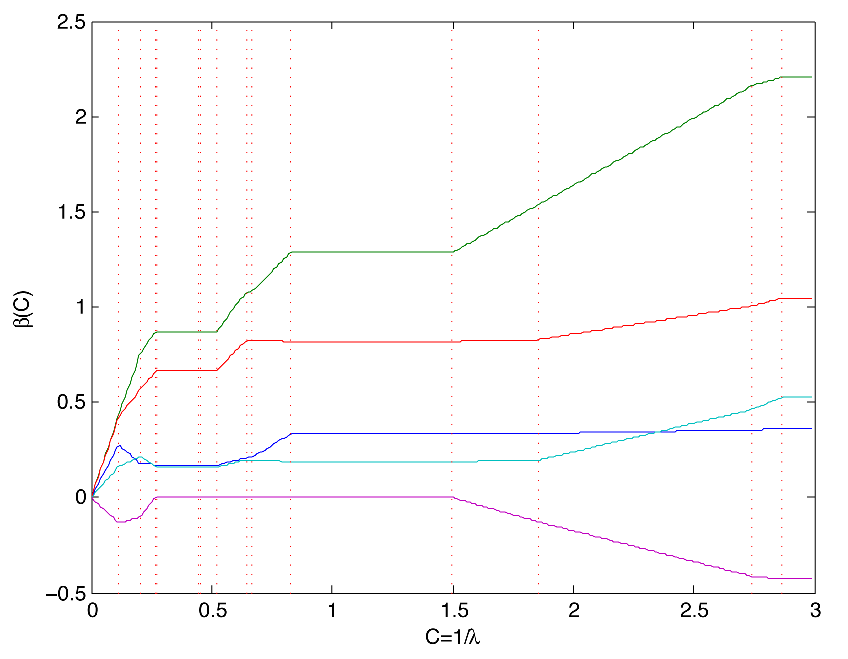
\includegraphics[width=0.7\textwidth]{./betaPath.pdf} 
      \caption{The path of $\beta$ for the simulated data.}
   \label{fig:betaPath}
\end{figure}
\end{center}


\subsection{Computation Complexity}
Hastie et al \cite{hastie2004entire} suggests the running time of their algorithm to be $O(n^2m+nm^2)$, where $m$ is the average size of the elbow $\mathcal E^l$. Since our algorithm is a variant of theirs (in particular, the core burden of the computation is still to solve the linear system which results in $O(m_l^3)$. Of course, we might have many of such systems the along the path), we conjecture our running time to be the same. We time our path algorithm for fitting the data in the previous section and the elapsed time is 1.01 secs on a 2.66 GHz Intel Core 2 Duo Mac OS machine. As a comparison, the running time for the brute-force algorithm is 66.27 secs for 300 points along the path. Note that the path algorithm gives the true path while the brute-force algorithm is still finding only a few snapshots of the path.  

%\subsection{Extension to Kernal} (You need to transform the uncertainty in the original data space into the kernal space)
%\note{in fitting the CEP data,  between 2.03 and 2.13 $\beta0$ value can be arbitrary}
\subsection{Matlab and R programs}
All the programs for this project are included in the {\tt zip} file submitted together with this hard copy. In particular, the matlab package {\tt svmIntervalPath} is the implementation of our path algorithm. Also, matlab and R code for testing and data analysis can be found in that file as well.


\section{Application to Variable Star Data Sets}
\subsection{Constructing the Intervals from the Time Series}
In certain applications, methods for constructing hyper-rectangles (or hyper-spheres) in feature space may be fairly straitforward. For example in El Ghaoui \cite{el2003robust}, the authors discuss applications to micro-array data where several replicates of some experiment are available, and a hyper-rectangle can be chosen to enclose all replicates.

With astronomy data there is no clearly correct way to construct intervals around features. A few possibilities include:
\begin{enumerate}
\item Make width of feature interval proportional to number of measurements in time series. Long time series will have small intervals around features, short time series will have wide intervals. For simple features, such as the standard deviation of the brightness measurements, making the interval width go down at rate root-n has a probabilistic interpretation via the central limit theorem.
\item Subsample the time series and derive features for each subsample. Represent observations as hyper-rectangles that contain features derived from every subsample (or a certain fraction of the subsamples).
\item Heuristically put intervals around observations with features that are wrong. For example, the amplitude of a star cannot be greater than 6 magnitudes, so any star with amplitude greater than 6 mags could be given an interval that contains values less than 6.
\end{enumerate}
In this work we take the second approach. While the first approach is attractive for simple features, many features (such as frequency) do not have a sqrt-n convergence to the true value. Further the irregular time sampling means that even simple features may not have a root-n convergence. The third approach involves a lot of domain knowledge and will change from application to application. Further, there is no guarantee that features within the range of what is physically possible are actually correct.

Figure \ref{fig:interval_construction} describes precisely how we subsample the time series and determine interval widths. The details of this procedure could be changed. For example one could bootstrap sample the time measurements, instead of subsampling contiguous sections. Certain computational considerations enter here. It takes around 1 second to derive features for an average length light curve. So sampling, say 20 times, could become prohibitively expansive if the data set is initially at the limits of what is computationally feasible.
\begin{figure*}[ht]
\begin{center}
{\small
\framebox[6in]{
\begin{minipage}[t]{5.8in}
% Insert here your text
\begin{center} \textbf{Constructing Hyper-rectangles from Time Series} \end{center}
\begin{enumerate}
\item Order the light curve measurements in time i.e. $\{(t_1,m_1,e_1),(t_2,m_2,e_2), \ldots , (t_l,m_l,e_l)\}$ where $t_i < t_j$ for $i < j$.
\item Slice each light curve into 5 contiguous sections, producing 5 time series. Slice 1 is $(t_i,m_i,e_i)$ for $\frac{0}{10}l \leq i \leq \frac{5}{10}l$, slice 2 is $\frac{1}{10}l \leq i \leq \frac{6}{10}l$, ect.
%% \begin{enumerate}
%% \item $\{(t_1,m_1,e_1), \ldots , (t_{l/2},m_{l/2},e_{l/2})\}$
%% \item $\{(t_1,m_1,e_1),(t_2,m_2,e_2), \ldots , (t_l,m_l,e_l)\}$
%% \end{enumerate}
\item Derive features for each of these slices.
\item Put the interval minimum at the lowest value of the feature for the 5 slices. Put the interval max at the maximum feature value across the 5 slices.
\end{enumerate}
\end{minipage}
}
}
\end{center}
\caption{Description of interval construction algorithm.\label{fig:interval_construction}}
\label{lb}
\end{figure*}

%% \begin{enumerate}
%% \item measurements in the middle of the light curve get used more often
%% \item sometimes the intervals do not contain the feature obtained when using the whole light curve. this is because taking shorter sections of light curves biases certain features high or low (frequency significance features tend to go down, should probably just get rid of these anyway)
%% \end{enumerate}
%% Bootstrap sampling might be a good approach, but this would destroy cadence sensitive features. So not sure what to do. This might be something interesting to discuss in the paper: \textbf{Determining feature error intervals for time series / image data is difficult.}




%% \section{Light Curves}

%% Figures \ref{fig:mira}, \ref{fig:cepheid}, \ref{fig:rrlyrae} show the light curves (i.e. time series) of three stars. Each is of a different class. The figures show the raw light curve (time on x-axis, magnitude on y-axis) and folded light curve (phase on x-axis, magnitude on y-axis). The phase is determined by computing a period (sometimes wrong!, for example figure \ref{fig:mira}) for each star, and then looking at the remainder of time divided by the period. The folded light curve often make the structure of the function much clearer.


%% \begin{figure}[h]
%%   \begin{center}
%%     \begin{includegraphics}[scale=.5]{4000.pdf}
%%       \caption{Light curve of a RR Lyrae AB variable star.\label{fig:rrlyrae}}
%%     \end{includegraphics}
%%   \end{center}
%% \end{figure}



%% \section{Initial Classification Work}

%% \subsection{Ignoring Errors}
%% I made a data set of 5508 of these light curves of class Mira, Classical Cepheid, and RR Lyrae AB. Random forest (a type of classifier) obtained a 0.55\% error rate, without using any feature error information. So the current classes may be too easy. I could generate features for some stars that belong to classes that are more similar to each other e.g. using stars from classes RR Lyrae C and RR Lyrae D (not used here) are a lot alike and would have much higher error rates.


\subsection{The Data Sets}
The first dataset analyzed contained two classes of Cepheids (CEP):  classical and [popII].  Each class consisted of $n=200$ observations and $p=58$ features so that each observation is hyperrectangle in $\mathbb{R}^{58}$. The second dataset consisted of two classes of RR,  RR Lyrae AB and RR Lyrae D, with the same values of $n$ and $p$.
\subsubsection{Preprocessing the data with quantile ranking}
A quantile ranking technique was used to normalize values in each feature dimension by reducing the effects of outliers. Viewing the interval data as a three-dimensional array, the end-slices corresponding to the lower- and upper-bounds of the confidence intervals were isolated and then concatenated together to yield a $2n\times p$ array whose values were then mapped to the standard normal distribution. Features containing all zeroes or some NaNs were removed from the dataset.

\subsection{Results}

\subsubsection{Performance}
The performance of the combined SVM model was compared to those of its degenerates by computing expected losses for multiple values of $\lambda$ and $\rho$.  For a given $(\lambda,\rho)$, the expected loss was computed by performing cross-validation in 90-10 splits so that the union of testing points across splits is the entire dataset and the intersection is disjoint. See surface plots of loss versus $(\lambda,\rho)$: for the CEP dataset, $\lambda\in \lbrace 0\rbrace\cup [0.375,0.750]$ and $\rho\in\lbrace 0\rbrace\cup [0.090,0.032]$ while for the RR dataset, $\lambda\in\lbrace 0\rbrace\cup [54,284]$ and $\rho\in\lbrace 0\rbrace\cup [0.375,0.750]$. Observe that $(\lambda^*,\rho^*)\neq (0,0)$ for both datasets, which implies that the combined model outperforms both of its degenerates. For the CEP dataset, the optimal $(\lambda^*,\rho^*)=(9,0.320)$ yielded 13.25\% classification error while for the RR dataset, $(\lambda^*,\rho^*)=(284,0.48)$ yielded 21.50\% classification error. THESE NUMBERS DON'T LOOK RIGHT, MUST RERUN analyze\_feature.m.

The curves of loss versus $\lambda$ and loss versus $\rho$ were also analyzed.  The loss versus $\lambda$ plot corresponds to the standard point SVM model in Hastie while the loss versus $\rho$ plot corresponds to the interval SVM model in El Ghaoui. Observe the convex-like curvatures, which suggest global minima and hence optimal $\lambda$ and $\rho$. 

\subsubsection{Feature selection as suggested by $||\beta||_0$ values}



\subsection{Conclusions}
\begin{enumerate}
\item constructing intervals is non-trivial in many high dimensional problems
\item not clear that this robust framework is ideal when new observation might have low error on certain features
\item kernels, are they possible to use
\item links to code / git repo
\end{enumerate}


\subsection{Appendix}
\begin{center}
\begin{figure}[!h]
   \centering
   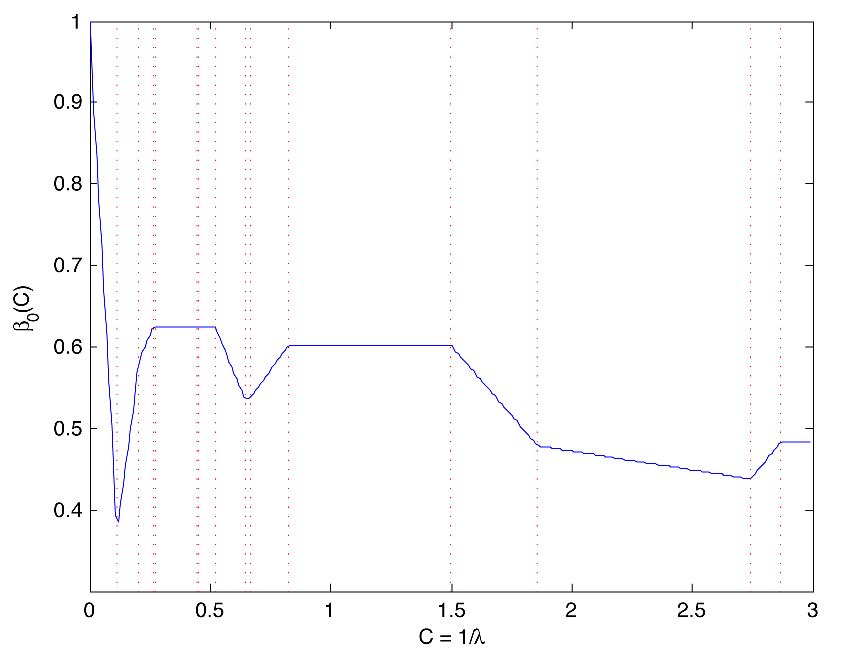
\includegraphics[width=0.7\textwidth]{./beta0Path.pdf} 
      \caption{The path of the intercept parameter $\beta_0$ for the simulated data. Notice that since $n_+=10>8=n_-$, by the first lemma, $\beta_0(0)=1$.}
   \label{fig:beta0Path}
\end{figure}
\end{center}

\begin{center}
\begin{figure}[!h]
   \centering
   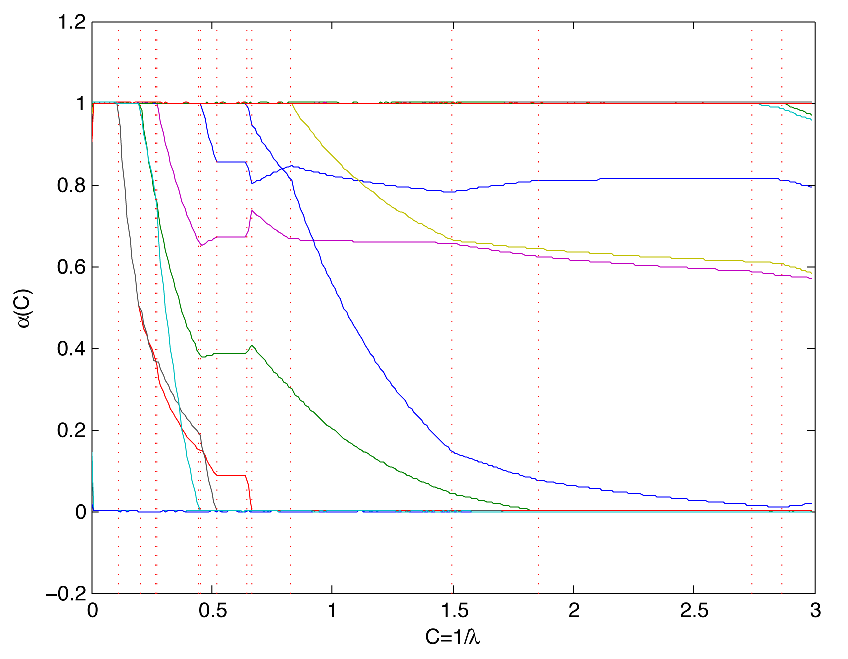
\includegraphics[width=0.7\textwidth]{./alphaPath.pdf} 
      \caption{The path of $\alpha$ for the simulated data.}
   \label{fig:alphaPath}
\end{figure}
\end{center}


\bibliographystyle{plain}
\bibliography{refs}



\end{document}
